%----------------------------Meta Data----------------------------%
\documentclass[xcolor=dvipsnames]{beamer} % xcolor for all colors

%Packages
\usepackage{pgfpages}
\usepackage{tikz}
%\usepackage{lcg}

% Packages for Algorithm
\usepackage{algorithm}
\usepackage{algpseudocode}

% Packages for Tables
\usepackage{booktabs} % For table commands
\usepackage{multirow} % For multirow

\usetheme{Frankfurt} % Theme with top navigation
%\usetheme{Madrid} % Theme with bottom information bar

\setbeamertemplate{navigation symbols}{} % Turn off navigation symbols.
\setbeamertemplate{footline}[page number] % Shows page number at the bottom right corner
\graphicspath{{Figures/}}

%Presentation Specific
\title{Beamer Template}
%\subtitle{Optional Subtitle}
\author{Marvin Buff}
\institute{University of Basel}
\date{13. February, 2017}

%Adds the navigation before every new section.
\AtBeginSection[]
{
  % Alternative Content between Chapters
  %\begin{frame}
  %  \frametitle{Table of Contents}
  %  \tableofcontents[currentsection]
  %\end{frame}
  
  \begin{frame}{Outline}
    \begin{center}
      \Huge \insertsection
    \end{center}
  \end{frame}
}

% Custom Makros
\newcommand{\light}[1]{\textcolor{gray}{#1}} % adds the command light to gray out text.
\newcommand{\ra}[1]{\renewcommand{\arraystretch}{#1}} % sets gap between rows, use \ra{1.3}
\newcommand{\sbc}{\setbeamercovered{transparent}}



%----------------------------Begin Document----------------------------%
\begin{document}

%-------------Frame::Title---------------%
\begin{frame}
  \titlepage
\end{frame}

%-------------Frame::Content---------------%
\begin{frame}{Outline}
  \tableofcontents%[pausesections]
\end{frame}


% Insert your Presentation HERE!
% Insert your Presentation HERE!
% Insert your Presentation HERE!


%-------------Section::Template-----------------%
\section{Example Section}
\subsection{Animation}%This adds a bullet on the navigation bar

\begin{frame}{Animation}
  \sbc{}
  \begin{block}{A basic block}<1->
    Another way to animate would be with: \textsc{\textbackslash{}pause}
  \end{block}
  \begin{exampleblock}{An exampleblock}<2->
    Or alternatively: \textsc{\textbackslash{}onslide<1-2>}
  \end{exampleblock}
  \begin{alertblock}{An alertblock}<3>
    But don't forget to set the beamer cover: \textsc{\textbackslash{}sbc}
  \end{alertblock}
\end{frame}

\subsection{Table}

\begin{frame}{Table}
  \begin{block}{Complex table}
    \begin{table}[H]\centering
      \ra{1.3}
      \begin{tabular}{l|c|cccc}
        % Title Row 1
        \multicolumn{1}{c}{Domain}& & \multicolumn{4}{c}{Solved Problems (\#)} \\ [0.5ex]
        \cmidrule(r){3-6}
        % Title Row 2
          & Algo & $h^0$ & $h^{max}$ & $h^m$ & $h^{lmCut}$ \\
        \toprule
        % Data Rows
        \multirow{2}{*}{Storage} & $A^*$ & \textbf{14} & \textbf{15} & \textbf{7} & \textbf{15} \\
          & \textsc{NBS} & 5 & 5 & 2 & 4 \\ 
        \bottomrule
      \end{tabular} 
    \end{table}
  \end{block}
  \begin{block}{Necessary Packages}
    \begin{itemize}
      \item booktabs %for table
      \item multirow %for multirow duhh..
    \end{itemize}
  \end{block}
\end{frame}

\subsection{Graphics}

%-------------Frame::Tikz-----------------%
\begin{frame}{Split Columns}
    \begin{columns}
    \begin{column}{0.5\textwidth}
          \begin{block}{Including Graphics}
              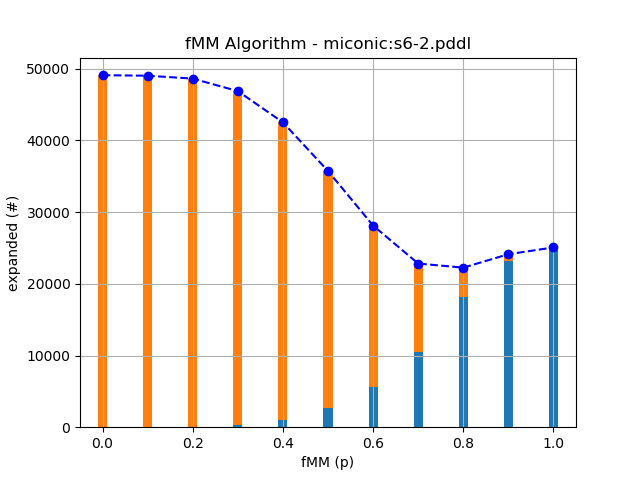
\includegraphics[width=1\textwidth]{test}
          \end{block} 
    \end{column}
    \begin{column}{0.5\textwidth}%
        \begin{exampleblock}{Tikz Example}
          \vspace{2mm}
          \begin{tikzpicture}[scale=0.55,
              state_style/.style={draw=black, shape=circle, minimum size=0.7cm},%inner sep = 0.5ex
              base_edge_style/.style={->, shorten >=1ex, shorten <=1ex},
              curved_style/.style={base_edge_style, bend right, bend angle=60}]
            \def\l{8}
            \node[state_style] at (0,0) (init) {$s_0$};
            \node[state_style] at (\l,0) (goal) {$s_G$};
            \node[state_style] at (\l/3,0) (forw) {$u$};
            \node[state_style] at (\l/3*2,0) (backw) {$v$};
            \draw[curved_style,<->] (init) to node[midway, fill=block body example.bg] {$C^*$} (goal);
            \draw[base_edge_style] (init) -- (forw);
            \draw[base_edge_style] (goal) -- (backw);
          \end{tikzpicture}
        \end{exampleblock} 
    \end{column}
    \end{columns}
\end{frame}

\subsection{Algorithm}
%-------------Frame::Algorithm-----------------%
\begin{frame}{Algorithm}
\begin{algorithm}[H]
\begin{algorithmic}[1]
\caption{Algorithm Title}
\State Put $s_0$ in $Open_F$ and $s_G$ in $Open_B$
\While{$Open_F$ and $Open_B$ are not empty}
    \State Among $u \in Open_F$ and $v \in Open_B$
    \State Select the pair $(u,v)$ with lowest $lb(u,v)$
    \If{$lb(u,v) \geq cost(U)$}
        \State \Return $U$
    \EndIf
    \State Expand both $u$ and $v$
    \If{new path from $s_0$ to $s_G$ is found}
        \State Update $U$ if new path is better than previous
    \EndIf
\EndWhile
\end{algorithmic}
\end{algorithm}
\end{frame}


\subsection*{Hidden Section}%Bullet point, but not in navigation
%-------------Frame::Proof-----------------%
\begin{frame}{Some Proof}
  \begin{theorem}
      $g(n) \leq \lfloor n/3\rfloor$
  \end{theorem}
  \begin{block}{Proof Sketch}
      \begin{enumerate}
      \item Every simple polygon can be guarded 
            with at most $\lfloor n/3\rfloor$ vertex guards.
      \item Some simple polygons require at least $\lfloor n/3\rfloor$ guards.
      \end{enumerate}
  \end{block}
\end{frame}

%-------------Section::Summary-------------%
\section*{Summary}
\subsection*{Summary}
\begin{frame}{Summary}
\begin{block}{Take Home Message}
  \begin{itemize}
      \vskip5pt
      \item \color{blue}The Art Gallery Problem \vskip5pt
      \item Fisk's Proof:  $g(n) \leq \lfloor n/3\rfloor$ \vskip5pt
      \item Triangulation
      \begin{itemize}
          \item Ear Clipping $O(n^2)$
          \item Sweep Line $O(n\ log\ n)$
          \item Las Vegas $O(n\ log^*\ n)$
          \item Polygon Cutting $O(n)$
      \end{itemize} \vskip15pt
  \end{itemize}
  \end{block}
\end{frame}

%-------------Frame::Questions-------------%
\begin{frame}
    \begin{center}
        \huge Questions? \normalsize
    \end{center}
\end{frame}


%-------------Appendix---------------%
\appendix
\section<presentation>*{\appendixname}
\subsection<presentation>*{For Further Reading}

\begin{frame}[allowframebreaks]
  \frametitle<presentation>{For Further Reading}
    
  \begin{thebibliography}{10}
    
  \beamertemplatebookbibitems
  % Start with overview books.
    
  \beamertemplatearticlebibitems
  % Followed by interesting articles. Keep the list short. 

  \bibitem{chen2017nbs}
    J. Chen, R. C. Holte, S. Zilles, N. Sturtevant
    \newblock Front-to-end bidirectional heuristic search with near-optimal node expansions.
    \newblock {\em IJCAI 2017}, pages: 489-495, AAAI Press. 
    
  \bibitem{eckerle2017sufficient}
    J. Eckerle, J. Chen, R. C. Holte, S. Zilles
    \newblock Sufficient conditions for node expansion in bidirectional heuristic search.
    \newblock {\em ICAPS 2017}, pages: 79-87, AAAI Press.  
  \end{thebibliography}
\end{frame}

\begin{frame}
    \begin{block}{Just an equation}
        \begin{equation}
            \textsf{log}^*\ n=\left\{
                \begin{array}{ll}
                  0 & \textsf{if }n \leq 1\\
                  1 + \textsf{log}^*~(\textsf{log }n) & \textsf{if } n > 1
                \end{array}
              \right.
        \end{equation}
    \end{block}
\end{frame}

\end{document}




